\documentclass[11pt]{scrreprt}

\usepackage[utf8]{inputenc}
\usepackage{ngerman}
%\usepackage{fullpage} % kleinere Ränder

\usepackage{comment} % für größere comments: \begin{comment} ... \end{comment}

% *** für eingefügte (pdf-)Grafiken
\usepackage[pdftex]{graphicx} 
\pdfminorversion=6
% ***

\usepackage{enumerate} %für geschachtelte Aufzählungen

% *** java listings
\usepackage{listings} 
\usepackage{courier} % courier schrift
\lstset{numbers=left, numberstyle=\tiny, basicstyle=\ttfamily  ,numbersep=5pt, tabsize=2}
\lstset{language=Java}
% ***

\usepackage{amsmath} %Matheformeln usw.
\usepackage{amssymb} %mathfrak

\usepackage[bookmarks=true]{hyperref} % hyperrefs aktivieren
\setcounter{secnumdepth}{3} %Numerierung bis Tiefe 3, also ab \paragraph ohne

%kitteh stuff
\linespread{1.25}


%*** title usw.
\title{MPD-Client}
\subtitle{Teil der Software Engineering II Studienarbeit WS 2011/2012, Inf 3}
\author{
Christopher Pahl,\\
Christoph Piechula,\\
Eduard Schneider,\\
und Marc Tigges}
\date{\today}
%***

%newcommands
%\newcommand{\neuesKommando}{Was zu tun ist}

\begin{document}
\maketitle
\tableofcontents
%\part{welcher Teil}
\chapter{Einleitung}
Ziel dieser Studienarbeit ist die vollständige Bearbeitung einer vorgegebenen Aufgabenstellung
nach einem selbst gewählten Vorgehensmodell. Die Aufgabenstellung schreibt vor, sich in einer
Gruppe zusammen zu finden und gemeinsam ein Software-Projekt zu bearbeiten und dabei strukturiert
 und professionell vorzugehen.
\begin{quote}
    \section{Rahmenbedingungen}
    \renewcommand{\labelitemi}{•}
    \begin{itemize}
        \item Persistente Datenspeicherung
        \begin{itemize}
	    \item Datei oder Datenbank (wenn schon bekannt)
        \end{itemize}
        \item Netzwerk-Programmierung
        \begin{itemize}
	    \item Eine verteilte Architektur (z.B.: Client/Server)
        \end{itemize}
        \item GUI
        \begin{itemize}
	    \item Swing
	    \item Web-basiert
        \end{itemize}
    \end{itemize}
    \section{Prozess-Anforderungen}
    \begin{itemize}
        \item Dokumentation aller Phasen(Analyse bis Testen)
        \item Auswahl eines konkreten Prozessmodells
        \begin{itemize}
	    \item Z.B. sd\&m, M3, RUP, Agile Methoden ...
	    \item Begründung (warum dieser Prozess passt zu Ihrem System)
        \end{itemize}
        \item Erstellung der Dokumente und UML-Diagramme
        \begin{itemize}
	    \item Visio
	    \item UML Werkzeuge (freie Wahl)
        \end{itemize}
        \item Fertige Implementierung 
        \begin{itemize}
	    \item Es kann mehr spezifiziert sein als implementiert
        \end{itemize}
        \item Spezifikation von Testszenarien
        \begin{itemize}
	    \item und der Beleg der erfolgreichen Ausführung
        \end{itemize}
        \item Lauffähiges System
    \end{itemize}
    \section{Mögliche Themen}
    \begin{itemize}
        \item CRM Systeme
        \begin{itemize}
	    \item Bibliothek
	    \item Musikshop
	    \item ...
        \end{itemize}
        \item Kommunikationssysteme
	\item Chat-Variationen (Skype, etc.)
	\item File-Verwaltungs-Systeme (eigener Cloud-Dienst)
	\item ...
    \end{itemize}
    \item Portale
    \begin{itemize}
	\item Mitfahrgelegenheit
	\item Dating-Agentur ;)
	\item ...
    \end{itemize}
\footnote{Folie Anforderungen, Autor Prof. Dr. Philipp Schaible, WS 2011/2012, Inf 3}
\end{quote}
Diese Arbeit ist wichtig, um den Studenten zu zeigen, wie man in einem Team zusammenarbeitet und nach
Software-Engineering-Methoden qualitativ hochwertige Software erstellt. Es geht im Folgenden um einen
Music-Player-Daemon-Client (Näheres bitte der Definition entnehmen). Dieses Thema wird behandelt, da es
alle Rahmenbedingungen abdeckt und im Interesse der Autoren liegt. Die Besonderheit liegt darin, dass
sich diese Software nach Fertigstellung auch wirklich anwenden lässt. Ziel ist die Erweiterung der
Fähigkeitn im Bereich der Software Engineering sowie das Erlernen von Methoden für wissenschaftliches Arbeiten.




\chapter{Wasserfallmodell mit Rücksprung}

\section{Definition}

\begin{quote}
Das Wasserfallmodell ist ein lineares (nicht iteratives) Vorgehensmodell in der Softwareentwicklung, bei dem der Softwareentwicklungsprozess in Phasen organisiert wird. Dabei gehen die Phasenergebnisse wie bei einem Wasserfall immer als bindende Vorgaben für die nächsttiefere Phase ein.\\

Im Wasserfallmodell hat jede Phase vordefinierte Start- und Endpunkte mit eindeutig definierten Ergebnissen. In Meilensteinsitzungen am jeweiligen Phasenende werden die Ergebnisdokumente verabschiedet. Zu den wichtigsten Dokumenten zählen dabei das Lastenheft sowie das Pflichtenheft. In der betrieblichen Praxis gibt es viele Varianten des reinen Modells. Es ist aber das traditionell am weitesten verbreitete Vorgehensmodell.\\

Der Name „Wasserfall“ kommt von der häufig gewählten grafischen Darstellung der fünf bis sechs als Kaskade angeordneten Phasen.
Ein erweitertes Wasserfallmodell mit Rücksprungmöglichkeiten (gestrichelt).\\

Erweiterungen des einfachen Modells (Wasserfallmodell mit Rücksprung) führen iterative Aspekte ein und erlauben ein schrittweises „Aufwärtslaufen“ der Kaskade, sofern in der aktuellen Phase etwas schieflaufen sollte, um den Fehler auf der nächsthöheren Stufe beheben zu können.\\

\footnote{Zitat aus:  http://de.wikipedia.org/wiki/Wasserfallmodell}
\end{quote}

\begin{figure}[h]
\centering
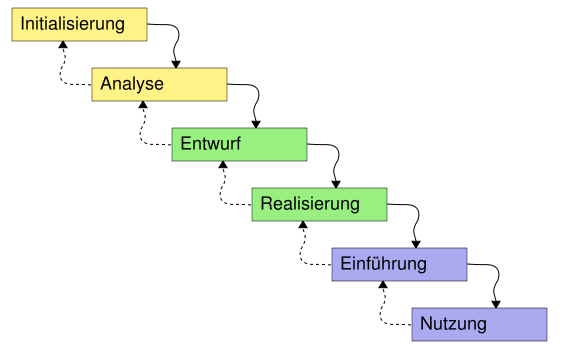
\includegraphics[scale=0.35]{567px-Wasserfallmodell.png}
\end{figure}
\footnote{Wasserfallmodell mit Rücksprung, Bild-Quelle: http://upload.wikimedia.org/wikipedia/commons/thumb/e/e5/Wasserfallmodell.svg/567px-Wasserfallmodell.svg.png}

\section{Warum dieses Modell?}
Wir haben uns für das Wasserfallmodell mit Rücksprung entschieden, weil dieses Modell alle Phasen der Entwicklung klar abgrenzt und sich optimal auf einen professionellen Softwareentwicklungsvorgang abbilden lässt.
Dieses Modell ermöglicht eine klare Planung und Kontrolle unseres Softwareprojekts, da die Anforderungen stets die gleichen bleiben und der Umfang einigermaßen gut abschätzbar ist.\\

Für die erweiterte Version dieses Modells, nämlich mit Rücksprung, haben wir uns entschieden, um ein paar Nachteile dieses Modells auszuhebeln. Beispielsweise sind die klar voneinander abgegrenzten Phasen in der Realität oft nicht umsetzbar. Des weiteren sind wir somit flexibler gegenüber Änderungen.

\chapter{Richtlinien}
\section{Programmierrichtlinien}
\renewcommand{\labelitemi}{•}
\begin{itemize}
\item Allman-Stil.
\item Tabstop = 4 Leerzeichen.
\item Keine globalen Variablen.
\item Sinnvolle Variablenbenennung, "'lowercase"'.
\item Klassenmethoden nur in Ausnahmefällen bzw. nur mit guten Gründen.
\item Valgrind darf keine Laufzeitfehler bringen, die nicht von Gtk oder anderen Bibliotheken stammen.
\item "'camelcase"' bei Objektnamen, C-Style bei Funktionsnamen - Präzise Namen.
\item Modulare Gestaltung.
\item Model-View-Controller Pattern
\item Code-Sauberkeit ist wichtiger als Code Performance.
\item "'make"' sollte keine Warnungen ausgeben, die man leicht umgehen könnte.
\item "'make test"' soll vollständig durchlaufen.
\end{itemize}
\subsection{Begründung}
Diese Programmierrichtlinen sorgen für ein einfaches, übersichtliches und einheitliches Arbeiten.
Jeder kann sich ohne größere Umstände in den Code eines anderen einlesen. Dies gewährleistet eine
hohe Wartbarkeit der Programm-Codes und beugt außerdem Fehlern vor. Das Programm ist leicht
erweiterbar ohne große Anpassungen vornehmen zu müssen.
\section{Toolauswahl}
\begin{itemize}
\item git
\item Glade
\item doxygen
\end{itemize}
\subsection{Begründung}
Git dient zur Versionsverwaltung. Glade bietet eine perfekte Trennung von der grafischen 
Oberfläche zum Kontrollkern des Programms außerdem kann mit Glade sehr
einfach eine grafische Oberfläche erstellt werden. Doxygen (Literate-Programming (KNUT))
\section{Bibliotheken}
\begin{itemize}
\item C++
\item gtkmm3 \footnote{http://www.gtkmm.org/de/index.html}
\item libmpdclient \footnote{http://www.musicpd.org/doc/libmpdclient/files.html}
\item libxml2 \footnote{http://xmlsoft.org/index.html}
\item libnotify \footnote{http://developer.gnome.org/libnotify/}
\item Avahi-glib \footnote{http://avahi.org/wiki/WikiStart\#WhatisAvahi}
\end{itemize}
\subsection{Begründung}
C++ wurde gewählt um die Fähigkeiten der Authoren zu erweitern. Außerdem gibt es für Java nur wenige
oder sehr alte Bibliotheken für dieses Projekt. Gtkmm3 bietet ein dynamisches Layout und ist
leichtgewichtiger als Qt, Swing ist aus Sicht der Authoren nicht geeignet. libmpdclient liefert eine 
eigene lowlevel C-Bibliothek.
Libxml2 liefert eine standardisierte config nach Xml-Standards, ist sehr leichtgewichtig und überall
installiert. Libnotify liefert Benachrichtigungen über interne Events und ist auf den meisten Linux
Distributionen verbreitet. Avahi-glib ist ein Interface für den Avahidaemon, der optional ist. Avahi 
dient als Server-Borwser, kann allerdings nur MPD Server finden, die mit einer zeroconf veröffentlicht 
wurden.\ \\ \\
Primäre Entwicklerplattform ist ein Unix-System nach Wahl.

\chapter{Definition}
Der MPD ist eine Client/Server-Architektur, in der die Clients und Server (MPD ist der Server)
über ein Netzwerk interagieren. MPD ist also nur die Hälfte der Gleichung. Zur Nutzung von 
MPD, muss ein MPD-Client (auch bekannt als MPD-Schnittstelle) installiert werden.
\section{Definition des MPD}
\begin{quote}
    Der Music Player Daemon (kurz MPD) ist ein Unix-Systemdienst, der das Abspielen von Musik auf 
    einem Computer ermöglicht. Er unterscheidet sich von gewöhnlichen Musik-Abspielprogrammen dadurch, 
    dass eine strikte Trennung von Benutzeroberfläche und Programmkern vorliegt. Dadurch ist die 
    grafische Benutzeroberfläche auswechselbar und auch eine Fernsteuerung des Programms über das 
    Netzwerk möglich. Die Schnittstelle zwischen Client und Server ist dabei offen dokumentiert und 
    der Music Player Daemon selbst freie und quelloffene Software.\ \\ \\
    Der MPD kann wegen seines geringen Ressourcenverbrauchs nicht nur auf Standartrechnern sondern 
    auch auf einem abgespeckten Netzwerkgerät mit Audioausgang betrieben werden und von allen Computern
    oder auch Mobiltelefonen / PDAs im Netzwerk ferngesteuert werden.\ \\ \\
    Es ist auch möglich den Daemon und den Client zur Fernsteuerung lokal auf dem gleichen Rechner
    zu betreiben, er fungiert dann als normaler Medienspieler, der jedoch von einer Vielzahl 
    unterschiedlicher Clients angesteuert werden kann, die sich in Oberflächengestaltung und Zusatzfunktionen
    unterscheiden. Mittlerweile existierten auch zahlreiche Clients, die eine Webschnittstelle bereitstellen.\ \\ \\
    Der MPD spielt die Audioformate Ogg Vorbis, FLAC, OggFLAC, MP2, MP3, MP4/AAC, MOD, Musepack und wave ab.
    Zudem können FLAC-, OggFLAC-, MP3- und OggVorbis-HTTP-Streams abgespielt werden. Die Schnittstelle kann
    auch ohne manuelle Konfigruation mit der Zeroconf-Technik angesteuert werden. Des Weiteren wird Replay
    Gain, Gapless Playback, Crossfading und das Einlesen von Metadaten aus ID3-Tags, Vorbis comments oder
    der MP4-Metadatenstruktur unterstützt.
    \footnote{Zitat aus: http://de.wikipedia.org/wiki/Music\_Player\_Daemon}
\end{quote}
\newpage
\subsection{Der MPD kann:}
\renewcommand{\labelitemi}{•}
\begin{itemize}
    \item Musik abspielen
    \item Musik kontrollieren und in Warteschlangen reihen 
    \item Musik Dateien dekodieren
    \item HTTP(Hyper Text Transfer Protocol) streamen
        \renewcommand{\labelitemi}{--}
        \begin{itemize}
            \item Eine HTTP-URL kann zur Warteschlange hinzugefügt oder direkt abgespielt werden.\\
        \end{itemize}
\end{itemize}

\subsection{Der MPD kann nicht:}
\begin{itemize}
    \item Album-Cover speichern
    \item Funktionen eines Equalizers bereitstellen
    \item Musik Taggen (Informationen aus dem Web suchen)
    \item Text für Playlist-Dateien parsen
    \item Statistische Auswertungen machen
    \item Musik visualisieren
    \item Funktionen eines Remote-File-Servers bereitstellen
    \item Funktionen eines Video-Servers bereitstellen
\end{itemize}
\section{Definiton des MPD-Client}
Der Music Player Daemon Client ist nun die Schnittstelle zum MPD. Über diesen Client kann der MPD
gesteuert werden. Es gibt viele verschiedene Clients mit unterschiedlichsten Funktionen, da der 
Client nicht auf den Funktionsumfang des MPD begrenzt ist. Das heißt im Klartext, dass der Client
zwar nur die Funktionen über das Netzwerk steuern kann, die vom MPD implementiert sind aber nicht, 
dass er deshalb auch keine lokalen Dienste bzw. Funktionen anwenden kann. So kann ein Client 
beispielsweise alle Funktionen lokal implementieren, die unter dem Punkt \"3.1.2 Der MPD kann nicht:\" 
erwähnt wurden.
\newpage
\section{Grafische Übersicht}
\begin{figure}[h]
    \centering
    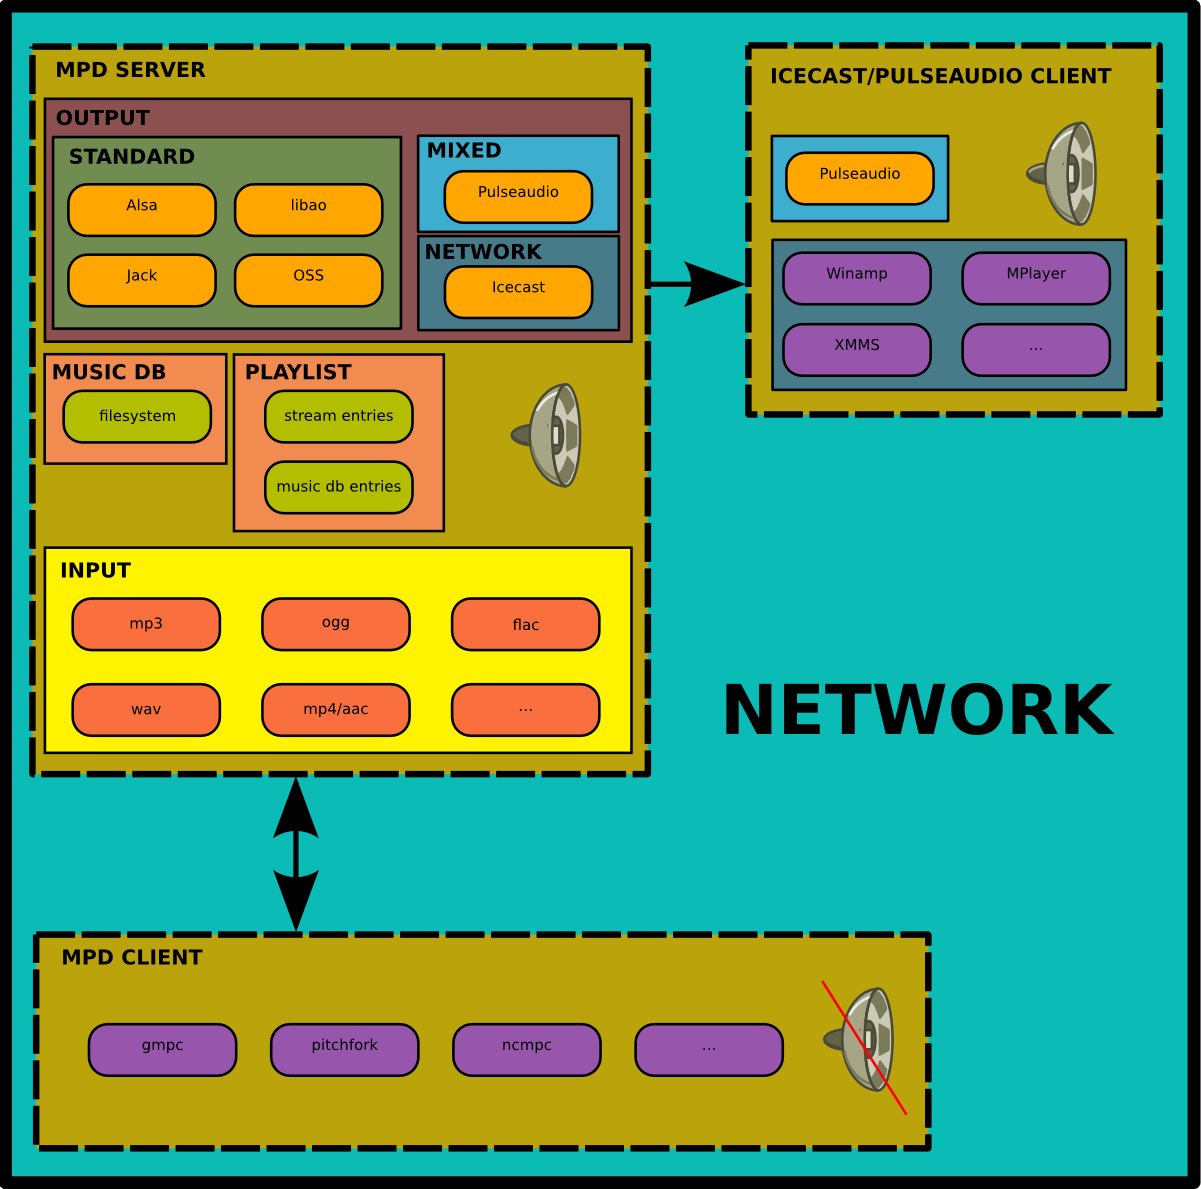
\includegraphics[scale=0.6]{Mpd-overview.png}
\end{figure}
\footnote{Bild-Quelle: http://images.wikia.com/mpd/images/6/68/Mpd-overview.png}
Der MPD-Server bekommt als Input mp3, ogg, flac, wav, mp4/aac,... Musik-Dateien die entweder in einer
Musik-Datenbank oder in Playlisten gespeichert sind. Der Standardoutput des MPD ist Alsa, libao, jack 
oder OSS, die Musik kann aber auch über einen Icecast oder Pulseaudio Clienten ausgegeben werden.
Der MPD-Client steuert den MPD-Server und hat selbst keinen Audio-Output.

\chapter{Lastenheft}
Bei der Erstellung dieses Lastenheftes wurde sich an folgendem Beispiel orientiert:
\begin{center}
http://www.stefan-baur.de/cs.se.lastenheft.beispiel.html?glstyle=2010
\end{center}
\section{Zielbestimmungen}
Welche Ziele sollen durch den Einsatz der Software erreicht werden?\ \\ \\
Dem einzelnen Benutzer soll das abspielen von Musik über eine Netzwerkverbindung ermöglicht
werden, dabei soll die Steuerung von einem lokalen Client übernommen werden. 
Die Musik wird dabei vom MPD Server in einer Datenbank gespeichert, der Rechner auf dem dieser
Dienst läuft ist auch primär für die Audioausgabe zuständig, desweiteren sind andere Audioausgabequellen
wie z.B. PulseAudio möglich.
Die Client-Rechner sollen die Ausgabe steuern und Abspiellisten auf dem Server verwalten
können. Die Bedienung soll für alle Benutzer sehr einfach und komfortabel über einen lokalen
Client realisiert werden. Bei jedem Start des Clients wird der Zustand des MPD-Servers ,,gespiegelt''.
\\ \\
Standardmäßig sollen den Benutzern folgende Funktionen zuf Verfügung stehen:
\renewcommand{\labelitemi}{•}
\begin{itemize}
        \item Abspielen von Musik
        \item Steuerung von Musik (Play, Stop, Skip, ...)
        \item Input-Stream via HTTP
        \item Erstellung und Verwaltung von Playlisten
        \item Verwaltung der der Audioausgabegeräte
\end{itemize}
Weitere Funktionen müssen modular integrierbar sein, allerdings müssen sie noch nicht implementiert
werden. Einige Beispiele für weitere Funktionen wären:
\begin{itemize}
	\item Finden von Album-Informationen \footnote{Unter Verwendung von: https://github.com/sahib/glyr}
	\item Speichern von Serveradressen
	\item Visualisierung der Musik
	\item Dynamische Playlisten
\end{itemize}
Die Systemsprache soll auf Englisch festgelegt werden.
\subsection{Projektbeteiligte}
Wer soll an dem Projekt teilnehmen?
\begin{itemize}
	\item Christopher Pahl
	\item Christoph Piechula
	\item Eduard Schneider
	\item Marc Tigges
\end{itemize}
\section{Produkteinsatz}
Für welche Anwendungsbereiche und Zielgruppe ist die Software vorgesehen?\ \\ \\
Der MPD-Client ist nicht auf bestimmte Gewerbe beschränkt, ein jeder soll diesen
Client verwenden können. 
\\
Die Software soll unter folgender Lizenz stehen:
Public License (GPL) Version 3 vom 29 Juni 2007.\ \\ \\
Definition der GPL v3:
\begin{center}
	http://www.gnu.org/licenses/gpl.html
\end{center}

\subsection{Anwendungsbereiche}
Einzelpersonen verwenden dieses System überall da, wo mit
einem Unix-artigen Betriebssystem Musik abgespielt werden soll.
Das wären z.B. Personal Computer, Musikanlagen, Laptops und evtl.
sogar diverse Smartphones möglich.

\subsection{Zielgruppen}
Personengruppen die komfortabel von überall aus auf ihre Musik und Playlist zugreifen
wollen ohne diese jedes mal aufwändig synchronisieren zu müssen (z.B. durch Abgleich von Datenträgern).\ \\ \\
Aufgrund der für das System vorgesehenen Betriebsumgebung sind ebenso Kenntnisse im Umgang mit Unix nötig.\ \\ \\
Der Benutzer muss die Systemsprache Englisch beherrschen.

\subsection{Betriebsbedingungen}
Das System soll sich bezüglich der Betriebsbedingungen nicht sonderlich von vergleichbaren Systemen bzw.
Anwendungen unterscheiden und dementsprechend folgende Punkte erfüllen:
\begin{itemize}
        \item Betriebsdauer: Täglich, 24 Stunden
        \item Keinerlei Wartung soll nötig sein
        \item Sicherungen der Konfiguration müssen vom Benutzer vorgenommen werden
\end{itemize}

\section{Produktumgebung}
\subsection{Software}
Softwareabhängigkeiten sollen durch den Entwickler bestimmt werden.
Dies gewährleistet, dass der Entwickler diesbezüglich nicht eingeschränkt wird
und somit mehr Möglichkeiten hat.

\subsection{Hardware}
Das Produkt soll möglichst wenig Anforderungen and die Hardware stellen, da
die Software eventuell auch auf sehr Hardwarearmen Geräten (wie z.B. Smartphones)
verwendet werden soll.

\subsection{Orgware}
Es soll nach Möglichkeit keine Orgware von nöten sein. Der Nutzer der Software soll sich
um möglichst wenig Nebenläufiges zu kümmern haben.

\section{Produktfunktionen}
Welche sind die Hauptfunktionen aus Sicht des Auftraggebers?

\subsection{Allgemein}
Beim ersten Start des Systems soll eine Standard-Konfiguration geladen werden und die Verbindungseinstellungen
zu einem MPD-Server müssen vorgenommen werden. Bei jedem weiteren Start soll die Konfiguration geladen werden,
die vom Benutzer erstellt wurde, falls keine Konfiguration gefunden wurde, oder diese korrumpiert ist,
so wird auf eine vom Client bereitgestellte Standardkonfiguration zurückgefallen. Der Benutzer soll sämtliche
Einstellungen selbstverständlich zu jeder Zeit über die Oberfläche des Clients ändern können.
Natürlich sollen alle üblichen Musik Abspielfunktionen vorhanden sein, dazu gehört Play, Stop, Previous
und Next. Aber auch erweiterte Funktionen wie Repeat, Consume und Random sollen einstellbar sein.
Der Benutzer soll über die Software direkten Zugriff auf das virtuelle Dateisystem des Servers haben, um nach Musik zu suchen und
diese abspielen zu können. Aus dem Dateisystem heraus soll der Nutzer ebenfalls die Möglichkeit haben, Musik-Dateien
direkt zu Playlisten und zur Warteschlange hinzuzufügen.
Verbindungseinstellungen müssen auf möglichst einfache Art und Weise vorgenommen werden können, wenn möglich
sollte dem Nutzer eine Liste von verfügbaren Servern angezeigt werden. 
Dem Nutzer soll ermöglicht werden, dass er nach bestimmten Titeln, Alben oder Interpreten suchen kann, da 
es mit dieser Software möglich ist, auch sehr große Musik-Datenbanken zu steuern.
Administratorfunktionen müssen nicht implementiert werden, das sie vom Unix-System übernommen werden.

\section{Produktdaten}
Welche Daten sollen persistent gespeichert werden?\ \\ \\
Die vom Benutzer vorgenommenen Verbindungseinstellungen und Client spezifischen Einstellungen,
sollen auf dem Rechner lokal und persistent gespeichert werden. Nur so kann ermöglicht werden,
dass nach jedem Start des Systems diese Einstellungen geladen und übernommen werden können.\ \\
Außerdem soll eine Log-Datei auf den einzelnen Rechnern angelegt werden, die dieses System
verwenden. Die Speicherung des Logs und der Konfiguration soll dabei dem XDG-Standard\footnote{http://standards.freedesktop.org/basedir-spec/basedir-spec-latest.html\#variables} entsprechen. 
In dieser Log-Datei werden Nachrichten des Systems gespeichert, um eventuelle Fehler
leicht finden und beheben zu können. Es soll stets der aktuelle Zustand des MPD Servers widergespiegelt werden.
\\
Dem Nutzer sollen viele verschiedene Informationen angezeigt werden, nicht nur Standardinformationen
wie Titel, Album und Interpret, sondern auch Musik-Qualität, -Länge und Lautstärke.
Es soll außerdem eine primitive Statistik implementiert werden die anzeigt, wie viele Lieder, Alben und
Interpreten in der Datenbank vorhanden sind, wie lange man schon mit dem Server verbunden ist und wie 
lange die gesamte Abspielzeit aller Lieder in der Datenbank dauert.\ \\
Eine Profilverwaltung muss nicht implementiert werden, dies wird bereits über die Unix Benutzerverwaltung geregelt.\ \\
Eine lokale Datenbank muss ebenfalls nicht vorhanden sein, dies wird durch den MPD-Server ermöglicht.\ \\

\section{Qualitätsanforderungen}
Die Software soll natürlich von hoher Qualität sein. Hierfür sollen folgende
Anforderungen erfüllt werden:\ 
\\
\\
Die Software soll korrekt sein, d. h. möglichst wenige Fehler enthalten.
Sie soll aber auch, für den Fall das dennoch Fehler auftreten, robust
und tolerant auf diese reagieren. Außerdem spielt die Wartbarkeit 
eine wichtige Rolle, falls sich die Softwareumgebung des MPD-Clients
ändert, muss dieser leicht angepasst werden können.
Der Client soll intuitiv und schnell bedienbar sein.
Der Hauptaugenmerk liegt dabei aber auf Ressourceneffizienz, vor allem soll dabei dabei 
das Netzwerk nicht stark beansprucht werden um auch bei langsamen Verbindungen den Client
bedienen zu können. Speicher und Recheneffizienz ist hierbei zwar von Belang, aber dennoch zweitrangig. 
Sollte es Funktionen geben, die nicht unter den Begriff "Standard" fallen, sollte eine knappe
und präzise Beschreibung der Funktion vorhanden sein.
Das Design der Software muss zwar ansprechend sein, ist im Endeffekt allerdings drittrangig.

\section{Ergänzungen}
\subsection{Realisierung}
Das System muss mit den Programmiersprachen C und/oder C++ realisiert werden. Dabei ist auf
Objektorientierung zu achten, um Modularität und Wartbarkeit gewährleisten zu können.
Es können beliebige Entwicklungsumgebungen verwendet werden, wobei allerdings auch ein Texteditor mit Syntaxhighlighting vollkommen ausreichend ist.
Um einfaches und sicheres Arbeiten ermöglichen zu können, soll die Versionsverwaltungssoftware \emph{git} benutzt werden, um die
Entwicklungsdateien zu speichern und zu bearbeiten. Zu dem Projekt soll eine ausführliche
Dokumentation erstellt werden, um dauerhafte Wartbarkeit und Anpassung des MPD-Clients gewährleisten
zu können, dazu gehören auch entsprechende Software-Diagramme (wie z.B. UML).
\subsection{Die nächste Version}
Aufgrund des modularen Aufbaus kann das System beliebig oft und in verschiedene Richtungen weiterentwickelt werden.
Weiter oben sind bereits Möglichkeiten für konkrete Erweiterungen aufgelistet.

\chapter{Pflichtenheft}
\section{Zielbestimmungen}
\subsection{Projektbeteiligte}
Wer soll an dem Projekt teilnehmen?
\begin{itemize}
        \item Christopher Pahl
        \item Christoph Piechula
        \item Eduard Schneider
        \item Marc Tigges
\end{itemize}
\subsection{Muss-Kriterien}
\renewcommand{\labelitemi}{•}
\begin{itemize}
	\item Server-Verbindung
	\item Client-Einstellungen
	\item Musik-Steuerung
\end{itemize}
\subsection{Wunsch-Kriterien}
\begin{itemize}
	\item Liedinformationen taggen
	\item Musikstatistik
	\item Album Covers
	\item Liedsuche
\end{itemize}
\subsection{Abgrenzungskriterien}
\begin{itemize}
	\item Musik-Visualisierung
	\item Chat
	\item Social-Network-Schnittstelle
\end{itemize}
\section{Produkteinsatz}
Welche Anwendungsbereiche (Zweck), Zielgruppen (Wer mit welchen Qualifikationen), Betriebsbedingungen (Betriebszeit,
Aufsicht)?\ \\ \\
Der MPD-Client ist nicht auf bestimmte Gewerbe beschränkt, ein jeder soll diesen Client
verwenden können. Grundlage für die Verwendung der Software ist die General Public License (GPL)
Version 3 vom 29 Juni 2007.\ \\ \\
Definition der GPL:
\begin{center}
http://www.gnu.org/licenses/gpl.html
\end{center}
\subsection{Anwendungsbereiche}
Einzelpersonen verwenden dieses System überall da, wo mit 
einem Unix-artigen Betriebssystem Musik abgespielt werden soll.
Das wären z.B. Personal Computer, Musikanlagen, Laptops und evtl.
sogar diverse Smartphones
\subsection{Zielgruppen}
Personengruppen die komfortabel von überall aus auf ihre Musik und Playlist zugreifen
wollen ohne diese jedes mal aufwändig synchronisieren zu müssen (z.B. durch Abgleich von Datenträgern).\ \\ \\
Es werden Basiskenntnisse zum Aufbau einer Netzwerkverbindung und zur Nutzung des Internets vorausgesetzt.
Aufgrund der für das System vorgesehenen Betriebsumgebung sind ebenso Kenntnisse im Umgang mit Unix nötig.\ \\ \\
Der Benutzer muss die Systemsprache Englisch beherrschen.
\subsection{Betriebsbedingungen}
Das System soll sich bezüglich der Betriebsbedingungen nicht sonderlich von vergleichbaren Systemen bzw.
Anwendungen unterscheiden und dementsprechend folgend Punkte erfüllen:
\begin{itemize}
	\item Betriebsdauer: Täglich, 24 Stunden
	\item Keinerlei Wartung soll nötig sein
	\item Sicherungen der Konfiguration müssen vom Benutzer vorgenommen werden
\end{itemize}
\section{Produktumgebung}
\subsection{Software}
\begin{itemize}
	\item Avahi Daemon
	\item MPD-Client
\end{itemize}
Ein MPD-Server ist nicht unbedingt von nöten.
\subsection{Hardware}
Minimale Hardwareanforderungen: 500 Mhz, 512MB Ram, Festplattenspeicher < 1MB
Empfohlene Hardwareanforderungen: 1 Ghz, 512MB Ram, Festplattenspeicher < 1MB
\subsection{Orgware}
\begin{itemize}
	\item git (Versionsverwaltungssoftware)
	\item cmake (Buildsystem)
	\item doxygen (Dokumentation)
	\item Editor nach Wahl
	\item Glade (GUI)
\end{itemize}
\section{Produktfunktionen}
Funktionen des MPD-Clients.\ \\ \\
Beim ersten Start des Systems soll eine Standard-Konfiguration geladen werden und die Verbindungseinstellungen
zu einem MPD-Server müssen vorgenommen werden. Bei jedem weiteren Start soll die Konfiguration geladen werden,
die vom Benutzer erstellt wurde, falls diese denn lokal gefunden werden kann. Der Benutzer soll sämtliche
Einstellungen selbstverständlich zu jeder Zeit ändern können.
\subsection{Starten und Beenden}
\begin{itemize}
	\item F\_0010 Der Benutzer kann das System zu jedem Zeitpunkt starten.
	\item F\_0011 Der Benutzer kann das System zu jedem Zeitpunkt beenden.
	\item F\_0012 Beim ersten Start wird ein Standart-System-Zustand geladen.
	\item F\_0013 Beim Beenden wird der aktuelle System-Zustand gespeichert.
	\item F\_0014 Bei jedem weiteren Start wird der letzte System-Zustand geladen.
\end{itemize}
\subsection{Abspielen von Musik (Buttons)}
\begin{itemize}
	\item F\_0020 Der Benutzer kann Musik abspielen (Play)
	\item F\_0021 Der Benutzer kann Musik stoppen (Stop)
	\item F\_0022 Der Benutzer kann Musik pausieren (Pause)
	\item F\_0023 Der Benutzer kann Musik vor und zurück schalten (Skip)
	\item F\_0024 Der Benutzer kann Musik vor und zurück spuhlen (Seek)
	\item F\_0025 Der Benutzer kann Musik zufällig abspielen (random)
	\item F\_0026 Der Benutzer kann Musik wiederholen (repeat)
	\item F\_0027 Der Benutzer kann Musik im Consume-Mode abspielen
	\item F\_0028 Der Benutzer kann Musik im Single-Mode abspielen
\end{itemize}
\subsection{Abspielen von Musik (Short-Cuts)}
\begin{itemize}
	\item F\_0030 Play 	(ctrl + G)
        \item F\_0031 Stop 	(ctrl + S)
        \item F\_0032 Previous 	(ctrl + P)
        \item F\_0033 Next	(ctrl + N)
	\item F\_0034 Random	(ctrl + Z)
	\item F\_0035 Single	(ctrl + Y)
	\item F\_0036 Repeate	(ctrl + R)
	\item F\_0037 Consume	(ctrl + T)
\end{itemize}
\subsection{Queue (Warteschlange)}
\begin{itemize}
	\item F\_0040 Der Benutzer kann einzelne Lieder aus der Queue entfernen
	\item F\_0041 Der Benutzer kann alle Lieder aus der Queue entfernen
	\item F\_0042 Der Benutzer kann kann die Queue als Playlist speichern
	\item F\_0043 Der Benutzer kann Interpret, Album und Titel beliebig anordnen
\end{itemize}
\subsection{Playlist}
\begin{itemize}
	\item F\_0050 Der Benutzer kann eine neue Playliste erstellen
	\item F\_0051 Der Benutzer kann eine vorhandene Playlist ersetzen
	\item F\_0052 Der Benutzer kann eine Playlist löschen
\end{itemize}
\subsection{Dateibrowser}
\begin{itemize}
	\item F\_0060 Der Benutzer kann durch sein Dateisystem navigieren
	\item F\_0061 Der Benutzer kann einzelne Dateien zur Queue hinzufügen
	\item F\_0062 Der Benutzer kann mehrere Dateien zur Queue hinzufügen
	\item F\_0063 Der Benutzer kann Dateien ersetzen
	\item F\_0064 Der Benutzer kann Die Anzeige aktualisieren
	\item F\_0065 Der Benutzer kann die Anzeige neu einlesen
\end{itemize}
\subsection{Statistik}
\begin{itemize}
	\item F\_0070 Der Benutzer kann eine gesamt Statistik einsehen
	\begin{itemize}
		\item Anzahl der Interpreten
		\item Anzahl der Alben
		\item Anzahl der Lieder
		\item Musiklänge der Datenbank
		\item Abspielzeit	
		\item Zeit Online bzw. mit MPD verbunden
		\item Letzter Datenbank-Update
	\end{itemize}
\end{itemize}
\subsection{Einstellungen}
\begin{itemize}
	\item F\_0080 Der Benutzer kann Netzwerk-Einstellungen vornehmen
	\begin{itemize}
		\item Server IP / Port
		\item Reconnect Timout in Sekunden
		\item Avahi-Browser (Serverauswahl)
		\item Autoconnect
	\end{itemize}
	\item F\_0081 Der Benutzer kann Playback-Einstellungen vornehmen	
	\begin{itemize}
		\item Crossface in Sekunden
		\item Musik beim verlassen stoppen
	\end{itemize}
	\item F\_0082 Der Benutzer kann Allgemein-Einstellungen vornehmen
	\begin{itemize}
		\item Notifications(libnotify) nutzen
		\item Tray-Icon anzeigen
	\end{itemize}	
	\item F\_0083 Der Benutzer kann die Standarteinstellungen wiederherstellen
\end{itemize}
\subsection{Lautstärke}
\begin{itemize}
	\item F\_0090 Der Benutzer kann die Lautstärke regeln
\end{itemize}
\subsection{Suchen}
Eine einfache Textsuche zum finden von Titeln, Alben oder Interpreten innerhalb der 
Abspiellisten wurde implementiert. Dabei springt die Markierung des Textes beim 
eingeben von Zeichen in die Suche zu der ersten übereinstimmenden Stelle in der 
Plaxlist des Clients. Erst beim bestätigen der Eingabe im Suchfeld wird die Auswahl 
gefilter.
\begin{itemize}
	\item F\_0110 Der Benutzer kann seine Queue durchsuchen.
	\item F\_0111 Der Benutzer kann sein Dateisystem durchsuchen.
\end{itemize}
\subsection{Sonstiges}
\begin{itemize}
	\item F\_0120 Verbinden	(ctrl + C)
	\item F\_0121 Trennen	(ctrl + D)
	\item F\_0122 Beenden	(ctrl + Q)
\end{itemize}
\subsection{Administrator-Funktionen}
Durch das Unix-artige System wird der Administrator-Zugriff geregelt. Sobald sich der Benutzer im Unix System
als Administrator befindet, kann er auch den MPD-Client administrieren. Ein zusätzlicher Administrator-Modus wurde also
nicht implementiert.
\section{Produktdaten}
\subsection{Anzeige}
\subsubsection{Titelleiste}
\begin{itemize}
	\item D\_0010 Titel
	\item D\_0011 Interpret
	\item D\_0012 Album
	\item D\_0013 Liedposition
	\item D\_0014 Lautstärke
\end{itemize}
\subsubsection{Queue}
\begin{itemize}
	\item D\_0020 Titel
	\item D\_0021 Interpret
	\item D\_0022 Album
\end{itemize}
\subsubsection{Playlist}
\begin{itemize}
	\item D\_0030 Name der Playlist
	\item D\_0031 Zuletzt geändert
\end{itemize}
\subsubsection{Statistik}
\begin{itemize}
        \item D\_0040 Anzahl der Interpreten
        \item D\_0041 Anzahl der Alben
        \item D\_0042 Anzahl der Lieder
        \item D\_0043 Musiklänge der Datenbank
        \item D\_0044 Abspielzeit
        \item D\_0045 Zeit Online bzw. mit MPD verbunden
	\item D\_0046 Letzter Datenbank-Update
\end{itemize}
\subsubsection{Fußleiste}
\begin{itemize}
	\item D\_0050 Qualität in Mhz
	\item D\_0051 Qualität in bit
	\item D\_0052 Qualität in kbit
	\item D\_0053 Outputart (Stereo, Sourround,...)
	\item D\_0054 Zeit aktuell von insgesamt
	\item D\_0055 Anzahl an Liedern
	\item D\_0056 Komplette Abspielzeit
	\item D\_0057 Lautstärke
\end{itemize}
\subsubsection{Sonstiges}
\begin{itemize}
	\item D\_0060 Nächster Song (Seitenleiste)
\end{itemize}
\subsection{Persönliches Profil}
Da die Software auf Unix-artige Systeme beschränkt ist, wurde keine Profil-Verwaltung implementiert. Die
verschiedenen Profile werden durch die verschiedenen Profile des gesamten Betriebssystems definiert und differenziert.
\subsection{Persönliche Datenbank}
Eine persönliche Datenbank ist lokal nicht vorhanden. Die Datenbank des Benutzers befindet sich auf dem MPD-Server.
Einzig und alleine modulare Erweiterungen des MPD-Clients können lokale Datenbank-Implementierungen erfordern.
\subsection{Persönliche Einstellungen}
Client Einstellungen werden lokal gespeichert.
\begin{itemize}
	\item config.xml
	\item ....
\end{itemize}
\section{Qualitätsanforderungen}
Die Software soll natürlich von hoher Qualität sein. Hierfür sollen folgende
Anforderungen erfüllt werden:
\subsection{Q\_0001 Korrektheit}
Die Software muss fehlerfrei und korrekt sein. Es wurden Testszenarien und Testfälle erstellt,
um Fehler zu finden und auszubessern. Aber auch wenn nach Veröffentlichung der Software ein 
Fehler gefunden werden sollte, wird dieser sofort ausgebessert. Bei schwerwiegenden Fehlern
werden die Nutzer direkt auf den Fehler aufmerksam gemacht.
\subsection{Q\_0002 Wartbarkeit}
Der Wartungsaufwandt der Software ist gering bis garnicht vorhanden. Ändert sich die Umgebungssoftware
(z.B. der MPD-Server) dann sind die Änderungen so geringfügig bzw. trivial, dass sie den MPD-Client 
nicht beeinflussen werden. Fehler der Software (sollten Fehler auftreten) wären leicht analysier- bzw.
prüfbar und natürlich auch leicht zu beheben. Zur Warbarkeit gehört ebenso die Modularität, d. h.
die Software ist technisch so realisiert, dass sie leicht erweitert werden kann, Stichwort Model View
Controller (MVC). Kritische Stellen werden von Fehlerbehandlungroutinen abgearbeitet.
Alle diese Routinen schreiben Meldungen in eine Log-Datei.
\subsection{Q\_0003 Zuverlässigkeit}
Das System funktioniert und reagiert tollerant auf fehlerhafte Eingaben bzw. fehlerhafte Benutzung.
Das Programm funktioniert sieben Tage die Woche und 24h am Tag und muss nicht abgeschaltet werden.
\subsection{Q\_0004 Effizienz}
Der MPD-Client ist technisch effizient. Das Programm ist schnell geladen und Eingaben des Benutzers
werden praktisch sofort ausgeführt. Es gibt so gut wie keine Wartezeiten, jedenfalls sind diese 
so genannten Reaktionszeiten für den Benutzer nicht merkbar. Selbst bei sehr großen Musik-Datenbanken
und Playlists benötigt das Programm kaum Rechenzeit und sonstige Hardware-resourcen.
\subsection{Q\_0005 Benutzbarkeit}
Die Software ist leicht verständlich und intuitiv bedienbar. Nötige Kenntnisse zur Nutzung des 
MPD-Clients sind leicht zu erlernen.
\subsection{Q\_0006 Design}
Das Design soll ansprechend und modern sein, allerdings wenn es Konflikte zwischen technischer Umsetzung 
und Design oder Effizienz und Design geben sollte, ist stets im Interesse der technischen Umsetzung bzw. 
der Effizienz zu entscheiden.
\section{Globale Testszenarien und Testfälle}
\subsection{Cxxtest}
CxxTest ist mit JUnit, CPPUnit oder xUnit zu vergleichen und somit ein leichtgewichtiges Framework für C++.
Der Vorteil gegenüber ähnlichen bzw. anderen Testmöglichkeiten sind die folgenden:
\begin{itemize}
	\item Es wird kein RTTI benötigt (Run-Time Type Information)
	\item Benötigt keine Member Template Funktionen
	\item Benötigt keine Exception-Behandlung
	\item Benötigt keine externen Bibliotheken (Memory Managment, File/Console I/O, Grafische Bibliotheken)
	\item Wird allein durch Header-Dateien (und ein Python-Skript) realisiert.
	\item Benötigt keine manuelle Regestrierung von Tests und Test-Suits
\end{itemize}
All diese Punkte machen CxxTest extrem portabel und nutzbar. Der Aufwandt zur Erstellung von Tests
wird minimiert.
\subsubsection{Testfälle}
\subsection{Testprotokoll}
Um Fehler aufzuspühren, die die grafische Oberfläche betreffen, wurd ein Testprotokoll erstellt in dem zunächst
alle möglichen Funktionen der grafischen Oberfläche aufgelistet werden. Außerdem müssen diese Funktionen mit 
anderen Funktionen kombiniert und mehrfach ausgeführt werden. Zu jedem dieser Fälle ist ein zu erwartendes Ergebnis
festzulegen und anschließend zu überprüfen ob das erwartete Ergebnis eingetroffen ist. Das eingetroffene Ergebnis
ist ebenfalls zu protokollieren.
\subsubsection{Abspielfunktionen}
Einfache Ausführung:\ \\ \\
\begin{tabular}[c]{|l|p{6cm}|c|}
\hline
\textbf{Testfall} & \textbf{Erwartetes Ergebnis} & \textbf{Ergebnis eingetroffen?}\\
\hline
Play & Musik spielt ab.\newline Play wird zu Pause. & Ja\\
\hline
Pause & Musik pausiert.\newline Pause wird zu Play. & Ja\\
\hline
Next & Nächstes Lied abspielen & Ja\\
\hline
Previous & Vorheriges Lied abspielen & Ja\\
\hline
Stop & Beende abspielen\newline Pause wird zu Play. & Ja\\
\hline
Skipping & An Liedposition springen & Ja\\
\hline
Random & Musik der Queue zufällig abspielen & Ja\\
\hline 
Repeat & Ein Lied wiederholen & Ja\\
\hline
Repeat all & Queue wiederholen & Ja\\
\hline
Consume Mode & Ein abgespieltes Lied entfernen & Ja\\
\hline
Single Mode & Ein Lied abspielen, dann Stoppen & Ja\\
\hline
\end{tabular}
\ \\ \\
Kombinierte Ausführung:\ \\ \\
\begin{tabular}[c]{|p{6cm}|p{6cm}|c|}
\hline
\textbf{Testfall} & \textbf{Erwartetes Ergebnis} & \textbf{Ergebnis eingetroffen?}\\
\hline
Play, Stop, Play & Musik spielt ab.\newline Musik stoppt.\newline Musik spielt ab. & Ja\\
\hline
Play, Pause, Play & Musik spiel ab.\newline Musik pausiert.\newline Musik spiel ab. & Ja\\
\hline
Next, Next & Skip weiter.\newline Skip weiter. & Ja\\
\hline
Previous, Previous & Skip zurück.\newline Skip zurück & Ja\\
\hline
Next, Previous & Skip weiter.\newline Skip zurück & Ja\\
\hline
Previous, Next & Skip zurück.\newline Skip weiter & Ja\\
\hline
Random, Repeat all & Musik der Queue zufällig abspielen\newline Queue wiederholen & Ja\\
\hline
Random, Consume Mode & Musik der queue zufällig abspielen\newline Ein abgespieltes Lied entfernen & Ja\\
\hline
Random, Single Mode & Musik der Queue zufällig abspielen\newline Ein Lied abspielen, dann stoppen & Ja\\
\hline
Consume Mode, Single Mode & Ein abgespieltes Lied entfernen\newline Ein Lied abspielen, dann Stoppen & Ja\\
\hline
Consume Mode, Repeat all & Kann nur einmal durchlaufen & Ja\\
\hline
\end{tabular}
\ \\ \\
Mehrfache Ausführung:\ \\ \\
\section{Entwicklungsumgebung}
\subsection{Software}
\begin{itemize}
	\item unix System
	\item MPD-Server	
	\item Avahi-Browser
\end{itemize}
\subsection{Hardware}
Keine Anforderungen spezifiziert
\subsection{Orgware}
\begin{itemize}
	\item git (Versionsverwaltungssoftware)
	\item cmake (Compiler)
	\item doxygen (Dokumentation)
	\item Editor nach Wahl
	\item Glade
\end{itemize}
\section{Glossar}

\chapter{Design-Dokument}
\section{Einleitung}
Dieses Dokument dient der Darstellung der Gesamt-Architektur des Software-Projekts "Freya-MPD-Client"
Zunächst werden einige UML-Diagramme zur Übersicht gezeigt und anschließend einzelne Funktionen der
Software genauer unter die Lupe genommen.\ \\
Im Anschluss daran wird die Benutzeroberfläche präsentiert und in Bereiche aufgeteilt genauer dargestellt.
Dabei werden alle Schaltflächen und Info-Panel genau erläutert.
Anschließend folgt eine Übersicht zu allen Short-Cuts die genutzt werden können.
Danach werden einige Use-Case-Fälle angeschaut, um genau zu verstehen, wie die Software mit dem Nutzer
interagiert und auf Befehle reagiert.
\newpage
\section{Softwarearchitektur}
\subsection{Architekutrübersicht}
\subsubsection{Namespace-Übersicht}
\begin{figure}[h]
\centering
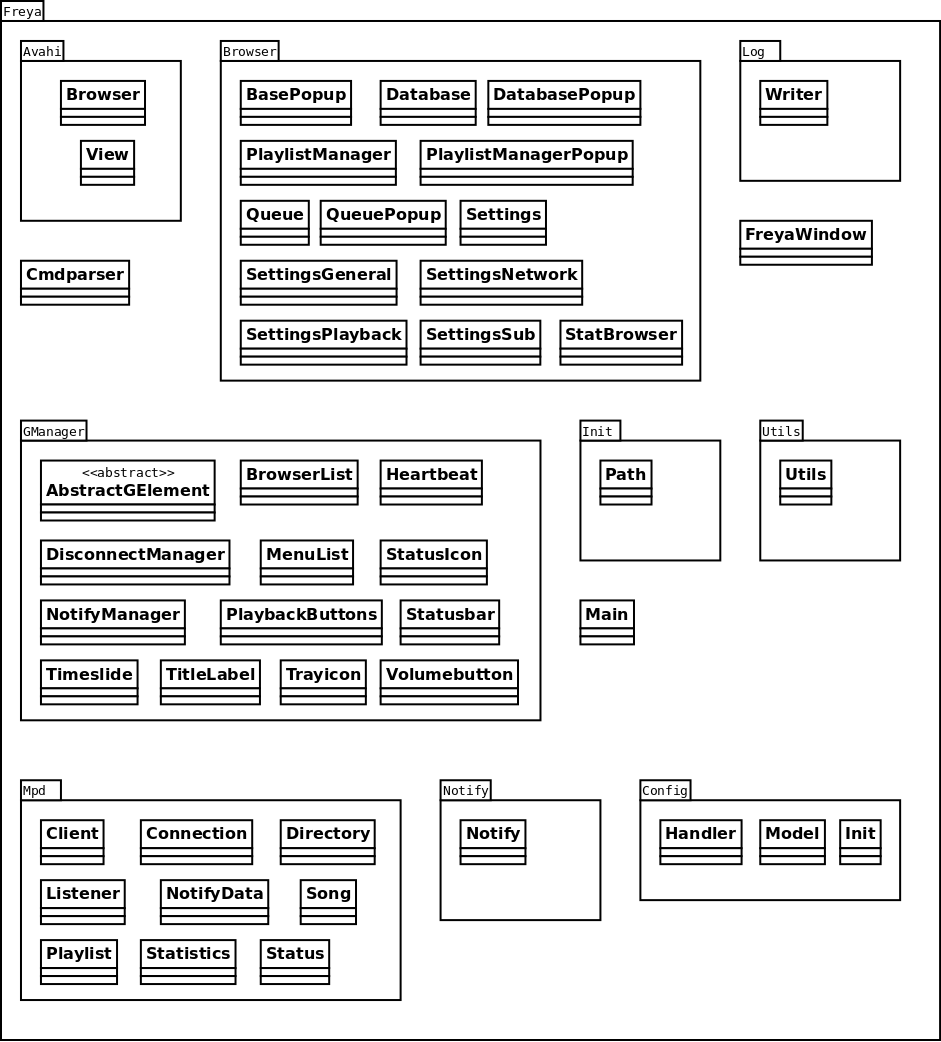
\includegraphics[scale=0.3]{Namespace_Uebersicht.png}
\end{figure}
\newpage
\subsubsection{Beschreibung}
\subsection{Funktionen}
\subsubsection{Beispiel-Abspielfunktionen}
\subsubsection{Beispiel-Playlist erstellen}
\subsubsection{Beispiel-Dateibrowser}
\subsection{Oberfläche}
\subsubsection{Titelleiste}
\subsubsection{Seitenmenü}
\subsubsection{Fußleiste}
\subsubsection{Anzeige}
\subsection{Short-Cuts}
\section{Use-Case-Fälle}
\subsection{Musik abspielen}
\subsection{Musik zufällig abspielen}
\subsection{Musik im Consume Mode abspielen}
\subsection{Playlist erstellen}



\end{document}
